%; whizzy paragraph -pdf xpdf -latex ./whizzypdfptex.sh
%; whizzy-paragraph "^\\\\begin{frame}\\|\\\\emtext"
% latex beamer presentation.
% platex, latex-beamer でコンパイルすることを想定。 

%     Tokyo Debian Meeting resources
%     Copyright (C) 2012 Junichi Uekawa
%     Copyright (C) 2014 Nobuhiro Iwamatsu

%     This program is free software; you can redistribute it and/or modify
%     it under the terms of the GNU General Public License as published by
%     the Free Software Foundation; either version 2 of the License, or
%     (at your option) any later version.

%     This program is distributed in the hope that it will be useful,
%     but WITHOUT ANY WARRANTY; without even the implied warreanty of
%     MERCHANTABILITY or FITNESS FOR A PARTICULAR PURPOSE.  See the
%     GNU General Public License for more details.

%     You should have received a copy of the GNU General Public License
%     along with this program; if not, write to the Free Software
%     Foundation, Inc., 51 Franklin St, Fifth Floor, Boston, MA  02110-1301 USA

\documentclass[cjk,dvipdfmx,12pt]{beamer}
\usetheme{Tokyo}
\usepackage{monthlypresentation}

%  preview (shell-command (concat "evince " (replace-regexp-in-string "tex$" "pdf"(buffer-file-name)) "&")) 
%  presentation (shell-command (concat "xpdf -fullscreen " (replace-regexp-in-string "tex$" "pdf"(buffer-file-name)) "&"))
%  presentation (shell-command (concat "evince " (replace-regexp-in-string "tex$" "pdf"(buffer-file-name)) "&"))

%http://www.naney.org/diki/dk/hyperref.html
%日本語EUC系環境の時
\AtBeginDvi{\special{pdf:tounicode EUC-UCS2}}
%シフトJIS系環境の時
%\AtBeginDvi{\special{pdf:tounicode 90ms-RKSJ-UCS2}}

\newenvironment{commandlinesmall}%
{\VerbatimEnvironment
  \begin{Sbox}\begin{minipage}{1.0\hsize}\begin{fontsize}{8}{8} \begin{BVerbatim}}%
{\end{BVerbatim}\end{fontsize}\end{minipage}\end{Sbox}
  \setlength{\fboxsep}{8pt}
% start on a new paragraph

\vspace{6pt}% skip before
\fcolorbox{dancerdarkblue}{dancerlightblue}{\TheSbox}

\vspace{6pt}% skip after
}
%end of commandlinesmall

\title{東京エリアDebian勉強会}
\subtitle{第118回 2014年10月度 OSC 2014 Tokyo/Fall 出張勉強会}
\author{岩松 信洋 / iwamatsu@debian.org}
\date{2014年10月18日}
\logo{
\includegraphics[width=8cm]{image200607/openlogo-light.eps}}

\begin{document}

\begin{frame}
\titlepage{}
\end{frame}

\begin{frame}{Agenda}
  \begin{itemize}
   \item Debian Update
   \item Debian 8 状況
   \item 質疑応答
   \item おしらせ
  \end{itemize}
\end{frame}

%
%\begin{block}{ブロック}
%\end{block}
%\begin{alertblock}{警告ブロック}
%\end{alertblock}
%\begin{exampleblock}{例ブロック}
%\end{exampleblock}
%

\begin{frame}{Who am I?}

\begin{itemize}
\item Debian Project 公式開発者
\begin{itemize}
\item linux kernel、ARM、SH4、Mactel チーム
\item Bluez, Mozc, OpenCV, Erlang
\end{itemize}
\item 普段は Linux カーネル、ブートローダ、BSP(Yocto, OE)の開発
\item U-Boot SH, rmobile メンテナ
\item Yocto Project meta-renesas メンテナ
\end{itemize}

\end{frame}

\emtext{Debian Updates}

\begin{frame}{ポイントリリース}

\begin{itemize}
\item Debian 7 更新状況 (Wheezy)
\begin{itemize}
\item 2014-04-26 Debian 7 更新: 7.5 リリース
\item 2014-07-12 Debian 7 更新: 7.6 リリース
\end{itemize}
\item Debian 6 更新状況 (Squeeze)
\begin{itemize}
\item 2014-07-19 Debian 6.0 更新: 6.0.10 リリース
\end{itemize}
\end{itemize}

\begin{center}
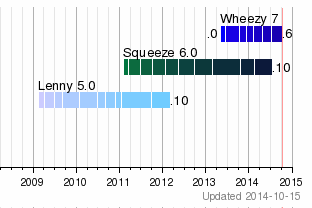
\includegraphics[scale=0.7]{image201410/debian-release-201410-cut.png}
\end{center}

\end{frame}

\begin{frame}[containsverbatim]{Long Term Support 開始}
\begin{itemize}
\item 2014/5/31 に Debian 6.x サポート終了
\item 2014/5/27 Debian 6.x 長期サポート (Long Term Support、LTS)開始
\begin{itemize}
\item Debian GNU/Linux 6.x
向けのセキュリティ更新を2016年2月6日まで提供(Squeezeのリリースから5年)
\item i386 と amd64 だけをサポート
\item 全てのパッケージがサポートされるわけではなく、サポート対象から外されるものもある
\item サポート対象外のパッケージはdebian-security-supportパッケージで管理されている
(check-support-status コマンドで確認できる)
\end{itemize}
\end{itemize}

\begin{commandline}
deb http://http.debian.net/debian/ squeeze main

deb http://http.debian.net/debian squeeze-lts main
\end{commandline}

\end{frame}

\begin{frame}{tracker.debian.org}
\begin{itemize}
\item Debian Package Tracking System(\url{packages.qa.debian.org})の置き換え
\item Django framework を使用
\end{itemize}

\begin{center}
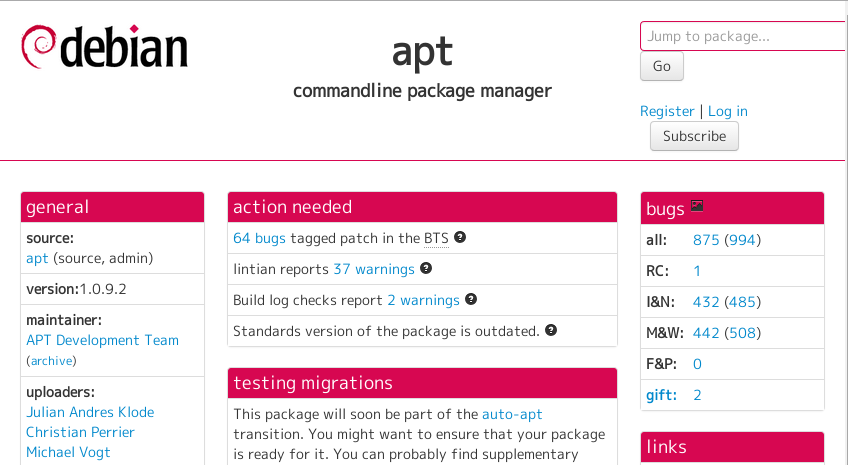
\includegraphics[scale=0.3]{image201410/tracker.png}
\end{center}

\end{frame}


\begin{frame}{Debconf 14}

\begin{center}

\includegraphics[scale=0.25]{image201410/debconf14-logo.png}
\end{center}

\begin{itemize}
\item 8月23日から31日まで、アメリカのポートランドで開催
\item 参加者は約300名(日本からの参加は2名)
\item カンファレンスのビデオや資料は \url{http://debconf14.debconf.org}
から参照可能
\item Debconf15 は ドイツのハイデルベルクで開催
\end{itemize}
\end{frame}

\emtext{Debian 8.0 状況}

\begin{frame}{近日フリーズ}
 
\begin{minipage}{0.55\hsize}
\begin{itemize}
\item 11/5 にフリーズ(予定)
\item フリーズ: パッケージの新しいバージョンへの更新を停止
\begin{itemize}
\item 9/5 にABI更新をフリーズ
\item 10/5 から testing へのマイグレーションを5日から10日に切り替え
\end{itemize}
\end{itemize}
\end{minipage}
\begin{minipage}{0.39\hsize}
\begin{center}
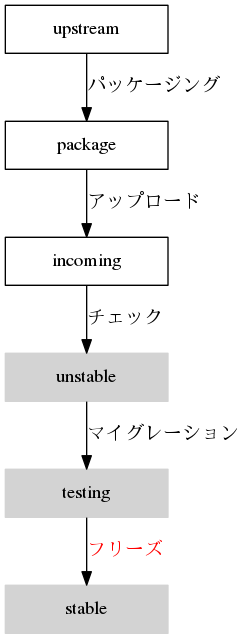
\includegraphics[scale=0.3]{image201410/lifesycle-package.png}
\end{center}
\end{minipage}
\end{frame}

\begin{frame}{リリースゴール}
\begin{itemize}
\item systemd
\item piuparts
\item SELinux
\item CrossToolchains
\item CrossBuildableBase
\item utf-8
\item debian/rules honor CC and CXX
\item Clang as secondary compiler
\item Security hardening build flags
\end{itemize}
\end{frame}


\begin{frame}{リリースゴールからはずされたもの}
\begin{itemize}
\item pkg-php-tools 移行(PEAR:PHP Extension and Application Repositoryサポート)
\end{itemize}
\end{frame}

\begin{frame}{サポートアーキテクチャ}

\begin{itemize}
\item IN: 未定
  \begin{itemize}
  \item arm64, ppcel64 はまだ決定ではない。11月1日の状況によって決まる
  %\item \url{https://lists.debian.org/debian-devel-announce/2014/09/msg00002.html}
  \item x32 は入らなかった模様。
  \end{itemize}
\item OUT: ia64、sparc、s390
\begin{itemize}
\item ia64 はdebian-ports でメンテナンス
\item s390 は s390x に移行
\end{itemize}
\end{itemize}

\end{frame}

\begin{frame}{デフォルト init システム}

\begin{itemize}
\item Linux のデフォルトの init システムが systemd に
\item minimal でインストールしても /sbin/init が systemd
\end{itemize}

\end{frame}

\begin{frame}{デフォルト Desktop Environment}

\begin{itemize}
\item GNOME
\item 他のDEが tasksel で選択可能に
\begin{center}
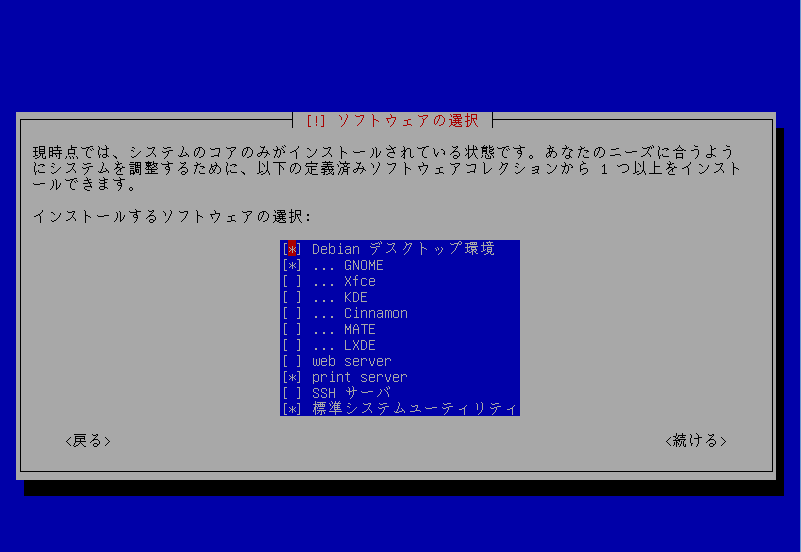
\includegraphics[scale=0.3]{image201410/instaler-tasksel.png}
\end{center}

\end{itemize}
\end{frame}

\begin{frame}{auto-removal によるリリース対策}
\begin{itemize}
\item RCバグに14日なにも進展がない場合、そのバグ
をもつパッケージは自動的にtestingから削除される。
\end{itemize}
\end{frame}

\begin{frame}{auto-removal によるリリース対策}
\begin{center}
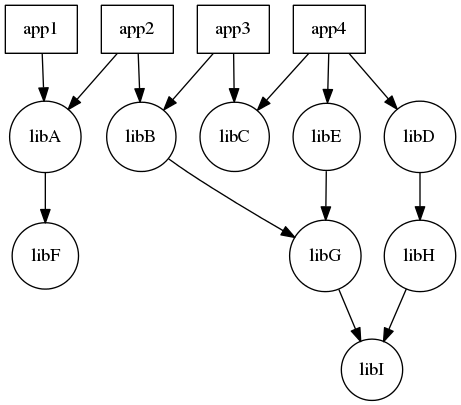
\includegraphics[scale=0.4]{image201410/auto-rm.png}
\end{center}
\end{frame}

\begin{frame}{auto-removal によるリリース対策}
\begin{center}
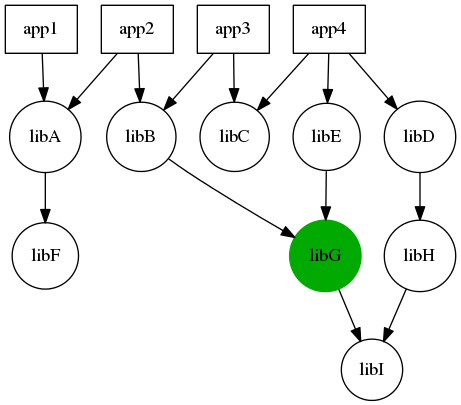
\includegraphics[scale=0.4]{image201410/auto-rm2.png}

libG が auto-rm される
\end{center}
\end{frame}

\begin{frame}{auto-removal によるリリース対策}
\begin{center}
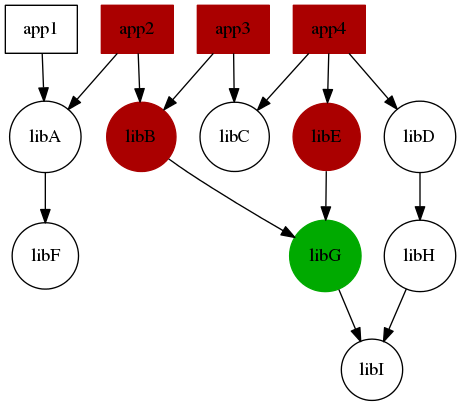
\includegraphics[scale=0.4]{image201410/auto-rm3.png}

libG に依存しているパッケージも auto-rm される
\end{center}
\end{frame}

\begin{frame}{auto-removal によるリリース対策}
\begin{itemize}
\item RCバグに14日なにも進展がない場合、そのバグ
をもつパッケージは自動的にtestingから削除される。
\item RCバグを持つパッケージとそれに依存しているパッケージが入らない可能性大
\item ただし、主要なパッケージは除く \\
主要パッケージ一覧\\
\url{https://udd.debian.org/cgi-bin/key_packages.yaml.cgi}
\end{itemize}
\end{frame}

\begin{frame}{主要ソフトウェアの更新状況}

\begin{itemize}
\item Linux kernel: 3.16.x (3.17.1)
\item kFreeBSD: 8,9,10 (10.1)
\end{itemize}

\end{frame}

\begin{frame}{主要ソフトウェアの更新状況}
\begin{itemize}
\item GNOME: 3.14 (3.14)
\item KDE: 4.14.1 (4.14.1)
\item Xfce: 4.10 (4.10)
\item LXDE: 0.7.1 (lxqt 0.8.0)
\item MATE: 1.8.0 (1.8.0)
\item Cinnamon: 2.2.16 (2.2.16)
\end{itemize}
\end{frame}

\begin{frame}{主要ソフトウェアの更新状況}
\begin{itemize}
\item Toolchain: GCC:4.9.1. binutils: 2.24.51, glibc: 2:19
\item LLVM: 3.4.2, 3.5.0 (3.5.0)
\item Perl: 5.20.1 (5.20.1)
\item Ruby: 2.1 (2.1)
\item Python2: 2.7.8 (2.7.8)
\item Python3: 3.4.2 (3.4.2)
\item PHP: 5.6.0 (5.6.2)
\item Lua: 5.2.3 (5.3.0 alpha)
\item ghc: 7.6.3 (7.8.3
\end{itemize}
\end{frame}

\begin{frame}{主要ソフトウェアの更新状況}
\begin{itemize}
\item Xorg: 1.16.1 (1.16.1)
\item Wayland: 1.6.0 (1.6.0)
\item systemd: 215 (216 )
\item Emacs: 24 (24.3)
\item Vim: 7.4.430 (7.4)
\item Pulseaudio: 5.0 ()5.0
\item Apache: 2.4.10 (2.4.10
\item VLC: 2.2.0~pre3 (2.1.5) 
\item zabbix: 2.2.6 (2.4.0)
\item rails: 4.1.6 (4.1.6)
\item django: 1.7 (1.7)
\item QEMU: 2.1 (2.1.2
\item lxc: 1.0.5 (1.0.6)
\end{itemize}

\end{frame}

\begin{frame}[containsverbatim]{Debian Installer Jessie Beta2}
\begin{itemize}
\item 10/6 に Debian Installer Jessie Beta 2 がリリース
\item arm64, ppcel64 イメージも追加
\item QEMU などで気軽に試せる
\end{itemize}
\end{frame}

\begin{frame}{まとめ}
\begin{itemize}
\item 11/5 にフリーズ予定
\item arm64, ppcel64 はまだ入るかわからない状態
\item デフォルトのinitシステムがsystemdになる
\item デフォルトのDEはGNOME。taskselから他のDEも選択可能に
\item RCバグを持つパッケージとそれに依存しているパッケージがJessie
に入らない可能性大
\item 主要パッケージは新しいものが入る(と思われる)
\item 既にインストーラがRCとしてリリース済み。テストできる環境は
整っている
\end{itemize}
\end{frame}

\begin{frame}{リリースに向けてお願い}
\begin{itemize}
\item 使っているパッケージでバージョンが古いものがありましたらご相談ください。ライブラリパッケージ以外は
まだアップデートできる可能性があります。
\item Debian 8.0で使いたいフリーソフトウェアがあったらご相談ください。まだ取り込まれる可能性があります。
\item テストにご協力ください。インストールレポート、ソフトウェア動作レポート、
未翻訳など報告していただけると非常に助かります。
\end{itemize}

\end{frame}

\begin{frame}[containsverbatim]{質問}

\begin{center}
なにか質問はありますか?
\end{center}

\end{frame}

\begin{frame}{おしらせ}
\begin{itemize}
\item ブース出展中
\begin{itemize}
\item Debian 起動 マシン展示(NUC, Minnowboard Max, BBB)
\item ステッカー、チラシ、インストーラCD配布
\item Debianに関する相談受付
\item GPGサイン、CAcertサイン
\end{itemize}
\end{itemize}

\end{frame}

\begin{frame}{次回の勉強会}
\begin{itemize}
\item 次回勉強会は 10/25(土)14:00-19:00 スクエアエニックスさん セミナールーム
\item Debian 8.0 (β版)インストール大会を行う予定
\item リリース前のDebian 8.0をインストールし、みんなで問題点などを洗い出す予定
\item 勉強会メンバがインストールのお手伝い
\item その他情報は Debian JP Project サイト \url{http://www.debian.or.jp}または Twitter:@debianjp にて
\end{itemize}
\end{frame}


\begin{frame}{利用画像等}
\begin{itemize}
\item
\url{http://upload.wikimedia.org/wikipedia/en/timeline/ed3c27abacc3656e55150a75faed2221.png}
\end{itemize}
\end{frame}

\end{document}

;;; Local Variables: ***
;;; outline-regexp: "\\([ 	]*\\\\\\(documentstyle\\|documentclass\\|emtext\\|section\\|begin{frame}\\)\\*?[ 	]*[[{]\\|[]+\\)" ***
;;; End: ***
